
\documentclass[12]{article}
\usepackage[utf8]{inputenc}
\usepackage{cite}
\author{par4111 \\ Adrià Cabeza, Xavier Lacasa \\ Departament d' Arquitectura de Computadors}
\title{Lab 2: Brief tutorial on OpenMP programming model }
\date{\today \\ 2018 - 19 PRIMAVERA}
\usepackage{graphicx}
%\usepackage[left=3.5cm, right=3.5cm]{geometry}
\usepackage{subcaption}
\usepackage{pgfplots}
\usepackage{listings}
\usepackage{xcolor}
\usepackage{float}
\lstset{
  basicstyle=\ttfamily,
  showstringspaces=false,
  commentstyle=\color{orange},
  keywordstyle=\color{blue},
	frame=tb,language=C,breaklines=true,numbers=none,  stringstyle=\color{red}, tabsize=3,   showstringspaces=false,
  columns=flexible, 
}
\begin{document}
\maketitle

\vspace*{\fill}
\begin{center}

\includegraphics[scale=0.5]{images/UPClogo.png}
\end{center}
\newpage
\tableofcontents
\newpage
\section{Introduction}

In this laboratory assignment we will learn the basics of OpenMP extensions to the C programming languge. At this moment we already know the hardware and tools we are going to use but this is the first approach to learn about the software needed to parallelize real applications. 

This is the scope of the next two sessions of PAR laboratory: introducing the  main components of the OpenMP programming model, from the simpler to the most complicated pragmas. 

\section{OpenMP questionnaire}

\subsection{Parallel regions}
\subsubsection{1.hello.c}
\textbf{1. How many times will you see the "Hello world!" message if the program is executed with \textit{./1.hello}?}

We see the message 24 times. This is due to the \textit{\#pragma omp parallel} call before \textit{printf("Hello world! \textbackslash n");}, which makes every available thread execute the \textit{printf}. In Boada 1, they happen to be 24 threads, and so the message is printed 24 times.

\textbf{2. Without changing the program, how to make it to print 4 times the \textit{Hello World!} message?}

By setting the number of threads available to 4, only 4 threads would execute the \textit{printf("Hello world! \textbackslash n");} line and so the message would be displayed only 4 times. We can accomplish this by adding \textit{num\_threads(4)} after \textit{\#pragma omp parallel}. Another way would be by using \textit{export OMP\_NUM\_THREADS=4} before the execution of \textit{1.hola}, so that only 4 threads are available.

\subsubsection{2.hello.c}
\textbf{1. Is the execution of the program correct? (i.e., prints a sequence of \textit{(Thid) Hello (Thid)
world!} being Thid the thread identifier). If not, add a data sharing clause to make it correct?} 

It is not correct, sometimes errors like \\
\textit{(2) Hello (1) Hello (1) world! (1) world!} \\
occur. These happen because the variable \textit{id} is declared before \textit{\#pragma omp parallel}, meaning all threads share it. Then what can happen is that for example thread 2 reads the variable \textit{id}, prints the \textit{"(2) Hello"} line, then thread 1 changes the variable, and when it is time to print the \textit{"(2) world!"}, thread 2 prints \textit{"(1) world!"} instead, because thread 1 assigned a new value before thread 2 was done.
\\
To make it correct, we can add the \textit{private(id)} tag to the \textit{\#pragma omp parallel num\_threads(8)} line, so that every thread has its own local value of the variable \textit{id}. This way, when they assign their own id, they do not change the value other threads are reading from the var \textit{id}.

\textbf{2. Are the lines always printed in the same order? Why the messages sometimes appear intermixed?
(Execute several times in order to see this).}
No, the lines are not always printed in the same order. This happens because threads do not get tasks assigned by \#id order, so whichever thread gets the task earlier in that execution will print earlier.
\\
Messages appear intermixed because even though we added the \textit{private(id)} tag, threads do not wait for other threads to finish their execution before printing their lines (that would be sequential instead of parallel). This way, one thread might print \textit{(id) Hello} and right then another thread's execution might start, printing \textit{(id) Hello} again with a different \textit{id}. After that, they both will finish with \textit{(id) world!} and messages will have been intermixed. To avoid this, we should make the execution of the other threads stop when one thread starts to print until it finishes (we could use the \textit{critical} construct), but that would make the execution sequential (with the added overhead of parallelization, even worse).

\subsubsection{3.how\_many.c}
Assuming the \textit{OMP NUM THREADS} variable is set to 8 with \textit{export OMP NUM THREADS=8}

\textbf{1. How many \textit{Hello world ...} lines are printed on the screen?}

20 \textit{Hello world ...} lines are printed on the screen. Each line is printed as many times as the number of threads available for the region of that line.

\begin{itemize}
    \item Hello world from the first parallel (8)!: 8 times
    \item Hello world from the second parallel (2)!: 2 times
    \item Hello world from the second parallel (3)!: 3 times
    \item Hello world from the third parallel (4)!: 4 times
    \item Hello world from the fourth parallel (3)!: 3 times 
\end{itemize}

\textbf{2. What does omp get num threads return when invoked outside and inside a parallel region?}

Outside a parallel region it returns the number of threads during the sequential execution, which is always just one.
\\
Inside a parallel region however, it returns the number of threads available (busy or not) for that region:
\begin{enumerate}
    \item For the first parallel region it returns all threads available for the program which are 8 (because of the \textit{export OMP\_NUM\_THREADS=8} restriction).
    \item  The second parallel region is inside a for loop which completes 2 iterations with \textit{i = 2 and 3}. Since the number of threads is set to \textit{i} at each iteration by calling \textit{omp\_set\_num\_threads(i)}, in the first iteration \textit{omp\_get\_num\_threads()} returns 2 and in the second and final one it returns 3. \\ Note that \textit{omp\_set\_num\_threads()} overrides the number of threads set by \textit{export OMP\_NUM\_THREADS=8}, which means that for the rest of the execution, unless otherwise specified, the number of available threads will be 3 (because the last call to \textit{omp\_set\_num\_threads(i)} was made in the second iteration, with \textit{i = 3}.)  
    \item Before the third parallel region, the \textit{\#pragma omp parallel} directive is extended by adding \textit{num\_threads(4)}, which overrides the number of available threads just for this entire parallel region to 4. This way \textit{omp\_get\_num\_threads()} returns 4.
    \item For this fourth parallel region the number of threads is not overriden, so it takes the value 3 (which is what \textit{omp\_get\_num\_threads()} returns) from the \textit{omp\_set\_num\_threads(3)} call in the for loop.
\end{enumerate}

\subsubsection{4.data\_sharing.c}
\textbf{1. Which is the value of variable x after the execution of each parallel region with different datasharing
attribute (shared, private, firstprivate and reduction)? Is that the value you would expect? (Execute several times if necessary)}

\begin{enumerate}
    \item After first parallel (shared) x's value keeps varying depending on the execution. It should be 120 as intended by the code because there are 16 threads (as set by \textit{omp\_set\_num\_threads(16)}) and $\sum_{i=0}^{15} i = 120$ , but its value after the execution is usually between 100 and 120. This variation occurs because all threads are sharing the same variable x, and to execute \textit{x+=omp\_get\_thread\_num();} they must first read the value of x and then write the result of the sum to it. When they do this, however, it can happen that for example thread 3 reads the value 10 in x, then thread 1 also reads the value 10, after that thread 3 updates x with 10+3=13 and thread 1, that has the old value of x, finally updates x with the value it knows: 10+1=11. And so x instead of being 10+3+1=14, is 11 because thread 1 did not notice thread 3's update of x. This happens quite randomly depending on the order of tasks assigned and threads occupation, so the final value of x keeps changing execution after execution.
    \item After second parallel (private) x's value is always 5. This is expected as x is assigned the value of 5 right before the second parallel region. Then at the time of declaration of the parallel region, x is declared private (\textit{\#pragma omp parallel private(x)}), which means that each thread will modify a local copy (to each thread) of x, but will in no case modify the shared value of the variable (private(x) also makes the local copies of x start without an initialised value instead of the value of x previous to the parallel region (5)). This way threads can't modify the value other threads have of x, but this also means that after the parallel region, unless strictly specified, the shared value of x is still the same as before executing the region, because none of the threads has written the value of their local copy of x to the shared variable x. This is why in the end of the second parallel region x is always equal to 5.
    \item After third parallel (firstprivate) x's value is also always 5. This is expected as well, since firstprivate(x) has the same behaviour as private(x) with the exception that firstprivate(x) initializes each local copy of x for each thread with the value that x had before the start of the parallel region. In this case, that value is 5. Still, this does not affect the value of x after the execution of the parallel region, but it changes the behaviour inside.
    \item After fourth parallel (reduction) x's value is always 125. This is correct because \textit{pragma omp parallel reduction(+:x)} is supposed to make local copies of x for each thread, just like private, but initializing them to the neutral element (for addition, this would be 0). Then each thread executes its instructions inside the parallel region and after that all local copies' values are added together with the initial value of x (which was 5). This is therefore equivalent to computing the following (remember there are 16 threads): 
    \begin{equation}
        5 + \sum_{i=0}^{15} i = 125
    \end{equation}
    And 125 is indeed what is printed after each execution for the fourth parallel region, so it is safe to assume it works as intended.
    
\end{enumerate}

\subsection{Loop parallelism}
\subsubsection{1.schedule.c}
\textbf{1. Which iterations of the loops are executed by each thread for each schedule kind?}
\begin{itemize}
\item \textbf{Schedule(static)}: There is an equal distribution of iterations for each thread. As we can see in the outputed execution of the loop, each of the four threads gets a chunk of 3 iterations, having in total of 12 iterations. 
\\
\begin{lstlisting}[frame=single]
Going to distribute 12 iterations with schedule(static) ...
Loop 1: (0) gets iteration 0
Loop 1: (0) gets iteration 1
Loop 1: (0) gets iteration 2
Loop 1: (1) gets iteration 3
Loop 1: (1) gets iteration 4
Loop 1: (1) gets iteration 5
Loop 1: (3) gets iteration 9
Loop 1: (3) gets iteration 10
Loop 1: (3) gets iteration 11
Loop 1: (2) gets iteration 6
Loop 1: (2) gets iteration 7
Loop 1: (2) gets iteration 8
\end{lstlisting}

\item \textbf{Schedule(static,2)}: There is also an equal distribution of iterations for each thread but in this case each thread is executing only 2 consecutive iterations of the for loop each time according to the thread order.
As we can see in the outputed execution of the loop, the iterations are given in chunks of size 2 and in order: thread 0 takes iteration 1 and 2, thread 1 takes iteration 2 and 3,...
\\
\begin{lstlisting}[frame=single]
Going to distribute 12 iterations with schedule(static, 2) ...
Loop 2: (3) gets iteration 6
Loop 2: (0) gets iteration 0
Loop 2: (0) gets iteration 1
Loop 2: (1) gets iteration 2
Loop 2: (1) gets iteration 3
Loop 2: (1) gets iteration 10
Loop 2: (1) gets iteration 11
Loop 2: (3) gets iteration 7
Loop 2: (0) gets iteration 8
Loop 2: (0) gets iteration 9
Loop 2: (2) gets iteration 4
Loop 2: (2) gets iteration 5
\end{lstlisting}


\item \textbf{Schedule(dynamic,2)}: Each thread is executing 2 consecutive iterations of the loop each time. However, the order is guided by the first thread that is free. 
As we can see in the outputed execution of the loop, the iterations are given also in chunks of size 2, but here they are not sorted, the assignment is given depending on the availability of the thread. 
\\
\begin{lstlisting}[frame=single]
Going to distribute 12 iterations with schedule(dynamic, 2) ...
Loop 3: (1) gets iteration 0
Loop 3: (1) gets iteration 1
Loop 3: (1) gets iteration 8
Loop 3: (1) gets iteration 9
Loop 3: (1) gets iteration 10
Loop 3: (1) gets iteration 11
Loop 3: (0) gets iteration 6
Loop 3: (0) gets iteration 7
Loop 3: (3) gets iteration 4
Loop 3: (3) gets iteration 5
Loop 3: (2) gets iteration 2
Loop 3: (2) gets iteration 3
\end{lstlisting}

\item \textbf{Schedule(guided,2)}: In this case, the size of each chunk is proportional to the number of unassigned iterations divided by the number of the threads. Therefore the size of the chunks decreases. The order is also given by the first who is free and the chunk-size specified (in this case 2) represents the minimum size of a chunk. 
\\
\begin{lstlisting}[frame=single]
Going to distribute 12 iterations with schedule(guided, 2) ...
Loop 4: (3) gets iteration 0
Loop 4: (3) gets iteration 1
Loop 4: (3) gets iteration 8
Loop 4: (0) gets iteration 2
Loop 4: (0) gets iteration 3
Loop 4: (0) gets iteration 10
Loop 4: (0) gets iteration 11
Loop 4: (1) gets iteration 6
Loop 4: (1) gets iteration 7
Loop 4: (2) gets iteration 4
Loop 4: (2) gets iteration 5
Loop 4: (3) gets iteration 9
\end{lstlisting}
\end{itemize}


\subsubsection{2.nowait.c}
\textbf{1. Which could be a possible sequence of printf when executing the program?}
\\
The nowait clause removes the synchronization time needed between threads. If we remove the clause, the threads don't wait the others to finish their parallel region executions so they continue executing code. That means that without the nowait clause the sequence of printf is printed randomly by both for loops (but respecting the code sequence in a thread). 
Let's see an example of the outputed execution (we changed the number of iterations of the code in order to be able to check our hypothesis): 
\\
\begin{lstlisting}[frame=single]
Loop 1: thread (0) gets iteration 0
Loop 1: thread (4) gets iteration 1
Loop 1: thread (7) gets iteration 2
Loop 2: thread (6) gets iteration 6
Loop 2: thread (5) gets iteration 7
Loop 1: thread (2) gets iteration 3
Loop 2: thread (3) gets iteration 4
Loop 2: thread (1) gets iteration 5

\end{lstlisting}

\textbf{2. How does the sequence of printf change if the nowait clause is removed from the first for directive?}
\\
If we did not have the nowait clause we would see first the sequence of printf done by the first loop and then the sequence done by the second loop:
In order to check if our hypothesis is correct let's see the outputed execution: 
\\
\begin{lstlisting}[frame=single]
Loop 1: thread (1) gets iteration 1
Loop 1: thread (0) gets iteration 0
Loop 2: thread (0) gets iteration 3
Loop 2: thread (1) gets iteration 2
\end{lstlisting} 
\textbf{3. What would happen if dynamic is changed to static in the schedule in both loops? (keeping the nowait clause)}
\\
 Even though we kept the nowait clause we would still get a correct printf sequence: first the first loop and then the second one. But why? The static clause creates a static scheduling type, that is, the iterations are grouped into chunks and each thread executes the threads in circular order. So there is implicitly an order into the static schedule. 

If we check the ouputed execution we can see that out hypothesis is true. 
\\
\begin{lstlisting}[frame=single]
Loop 1: thread (0) gets iteration 0
Loop 1: thread (3) gets iteration 3
Loop 1: thread (2) gets iteration 2
Loop 1: thread (1) gets iteration 1
Loop 2: thread (0) gets iteration 4
Loop 2: thread (2) gets iteration 6
Loop 2: thread (1) gets iteration 5
Loop 2: thread (3) gets iteration 7
\end{lstlisting}

\subsubsection{3.collapse.c}
\textbf{1. Which iterations of the loop are executed by each thread when the collapse clause is used?}
\\
The collapse clause will parallelize more than one level of the loop. So each thread will execute consecutively a set of consecutive iterations that corresponds to the sequential iterations of the loops combined. To sum up, the iterations are in groups like it was only one loop. 
\\
\begin{lstlisting}[frame=single]
(0) Iter (0 0)
(0) Iter (0 1)
(0) Iter (0 2)
(0) Iter (0 3)
(1) Iter (0 4)
(1) Iter (1 0)
(1) Iter (1 1)
(3) Iter (2 0)
(3) Iter (2 1)
(3) Iter (2 2)
...
\end{lstlisting}
\textbf{2. Is the execution correct if the collapse clause is removed? Which clause (different than
collapse) should be added to make it correct?}
\\
If we delete the clause the execution is not correct because only the i is protected and the j is shared. In order to solve it we could make private the variable j to avoid having different iterations of the loop overriding the variable j.
\\
\begin{lstlisting}[frame=single]
int main()
{
    int i,j;

    omp_set_num_threads(8);
    #pragma omp parallel for private(j)
    for (i=0; i < N; i++) {
          for (j=0; j < N; j++) {
          int id=omp_get_thread_num();
          printf("(%d) Iter (%d %d)\n",id,i,j);
        }
    }

    return 0;
}

\end{lstlisting}
 
\subsection{Synchronization}
\subsubsection{1.datarace.c} 
\textbf{1. Is the program always executing correctly?}
\\
No. There is a data race.
\\
\medskip

\textbf{2. Add two alternative directives to make it correct. Explain why they make the execution correct.}
\\
\medskip

\begin{Large}
Alternative 1
\end{Large}
\\
\begin{lstlisting}[frame=single]
int main()
{

    int i, x=0;
    omp_set_num_threads(8);
    #pragma omp parallel private(i)
    {
    	int id = omp_get_thread_num();
    	for (i=id; i < N;i+=8) {
        	#pragma omp critical
        	x++;
    	}
	}

    if (x==N) printf("Congratulations!, program executed correctly (x = %d)\n", x);
    else printf("Sorry, something went wrong, value of x = %d\n", x);

    return 0;
}  
\end{lstlisting}  
This version protects the operation x++, where we had the data race. We created a critical region that only one thread can execute at once.
\\
\\
\medskip
\begin{Large}
Alternative 2
\end{Large}
\\
\begin{lstlisting}[frame=single]
int main()
{

    int i, x=0;
    omp_set_num_threads(8);
    #pragma omp parallel private(i)
     {
    	int id = omp_get_thread_num();
   		for (i=id; i < N;i+=8) {
        	#pragma omp atomic
        	x++;
    	}
	}

    if (x==N) printf("Congratulations!, program executed correctly (x = %d)\n", x);
    else printf("Sorry, something went wrong, value of x = %d\n", x);

    return 0;
}
\end{lstlisting}
Like in the previous version, here we are also protecting the operation x++, in this case we made the operation x++ indivisible using the atomic pragma directive, forcing to make the read and write operations on one thread before allowing another thread to access the variable. 

\subsubsection{2.barrier.c}
\textbf{1. Can you predict the sequence of messages in this program? Do threads exit from the barrier
in any specific order?} 
\\
Not at all.
A barrier defines a point in the code wher all the active threads will stop unitl all threads have arrived at that point. So we can suppose that we will get all the last messages about being awake at the same time. Also, we can say that all the messages about going to sleep are going to be printed before the ones about being awake, and the sequence of threads being awake can be predicted (because of the seconds that each thread is going to sleep). Moreoever, the threads don't exit the barrier in any specific order. 

\subsubsection{3.ordered.c}
\textbf{1.Can you explain the order in which the \textit{Outside} and \textit{Inside} messages are printed?} 
\\
The orderer clause works like this: different threads execute concurrently until they encounter the ordered region, which is executed sequentially in the same order as it would get executed in a serial loop. So, the order in which the \textit{Outside} and \textit{Inside} messages are printed is because of the fact that the inside message is inside the ordered region (that is executed sequentially) and the outside message is outside that region where all the different threads are executing concurrently. 
\\
\begin{lstlisting}[frame=single]
Before ordered - (0) gets iteration 0
Inside ordered - (0) gets iteration 0
Before ordered - (4) gets iteration 1
Inside ordered - (4) gets iteration 1
Before ordered - (4) gets iteration 3
Before ordered - (0) gets iteration 2
Inside ordered - (0) gets iteration 2
Before ordered - (2) gets iteration 5
Before ordered - (3) gets iteration 4
Before ordered - (5) gets iteration 6
Before ordered - (0) gets iteration 7
Inside ordered - (4) gets iteration 3
Before ordered - (6) gets iteration 10
Before ordered - (7) gets iteration 9
Before ordered - (1) gets iteration 8
Inside ordered - (3) gets iteration 4
Inside ordered - (2) gets iteration 5
Before ordered - (2) gets iteration 13
...
\end{lstlisting}

\textbf{2. How can you ensure that a thread always executes two consecutive iterations in order during the execution of the ordered part of the loop body?}
\\
Changing from schedule dynamic to schedule(dynamic,2)

\subsection{Tasks}
\subsubsection{1.single.c}
\textbf{1. Can you explain why all threads contribute to the execution of instances of the single worksharing
construct? Why are those instances appear to be executed in bursts?}

All threads contribute because \textit{\#pragma omp parallel} is called before the for loop, which means that all threads available will execute it, but inside the for loop there is a \textit{\#pragma omp single nowait} call which causes the instruction inside the for loop to be executed only once, by an available thread (this is because of \textit{single}). The \textit{nowait} call makes other threads continue their execution without waiting for the thread executing the \textit{single} instruction to end. \\
To sum up, what happens is that all threads execute the for loop but each iteration is assigned once and only to one thread available. So because there are 4 threads available (due to \textit{omp\_set\_num\_threads(4)}), the first 4 iterations are executed each by only one thread and all at once (because of the \textit{nowait}). Then the 4 threads wait 1 second (because of the \textit{sleep(1)} call), which explains the bursts, and do the same again until the for loop ends.

\subsubsection{2.fibtask.c}
\textbf{1. Why all tasks are created and executed by the same thread? In other words, why the program
is not executing in parallel?} 

Because there is not a \textit{\#pragma omp parallel} call before the while loop (or anywhere at all), meaning there is only one thread creating tasks and only one thread (the same that created them) available to complete them. 

\textbf{2. Modify the code so that the program correctly executes in parallel, returning the same answer that the sequential execution would return.}
To accomplish this we first need to make the parallelization possible by adding \textit{\#pragma omp parallel} before the while loop. If we left it like this, it would be incorrect because the every task would be created for every thread available, meaning we would repeat tasks as many times as threads available. To avoid this we add a \textit{\#pragma omp single} instruction before the while loop too, in order for the tasks to only be created by one thread but executed by whichever thread is available. We are now almost there, but there is a little problem with the variable \textit{p}: since it is a pointer that is passed to the function that each task computes, we need to make it private so that when a task is created with a certain value of \textit{p}, this value is not changed by the next iteration of the while loop. Also, since the initial value of \textit{p} is assigned out of the while loop, we want to make sure that, when made private, \textit{p} is still initialised with the value desired (we accomplish this by calling \textit{\#pragma omp parallel firstprivate(p)}). \\
Now the execution would be correct and the result we would get is 75025, which is indeed the 25th number in the Fibonacci series.\\
\medskip

This is the modified code (only the main() has been modified):
\medskip
\begin{lstlisting}[frame=single]
    int main(int argc, char *argv[]) {
        struct node *temp, *head;

        printf("Staring computation of Fibonacci for numbers in linked list \n");

        p = init_list(N);
        head = p;

        #pragma omp parallel firstprivate(p)
        {
            #pragma omp single
            {
                while (p != NULL) {
                    printf("Thread %d creating task that will compute %d\n", omp_get_thread_num(), p->data);
                    #pragma omp task 
                    { processwork(p); }
                    p = p->next;
                }
            }
        }
        printf("Finished creation of tasks to compute the Fibonacci for numbers in linked list \n");

        printf("Finished computation of Fibonacci for numbers in linked list \n");
        p = head;
        while (p != NULL) {
        printf("%d: %d computed by thread %d \n", p->data, p->fibdata, p->threadnum);
        temp = p->next;
        free (p);
        p = temp;
        }
        free (p);

        return 0;
    } 
\end{lstlisting}

\bigskip

And this is the obtained output:
\medskip
\begin{lstlisting}[frame=single]
    Staring computation of Fibonacci for numbers in linked list 
    Thread 0 creating task that will compute 1
    Thread 0 creating task that will compute 2
    Thread 0 creating task that will compute 3
    Thread 0 creating task that will compute 4
    Thread 0 creating task that will compute 5
    Thread 0 creating task that will compute 6
    Thread 0 creating task that will compute 7
    Thread 0 creating task that will compute 8
    Thread 0 creating task that will compute 9
    Thread 0 creating task that will compute 10
    Thread 0 creating task that will compute 11
    Thread 0 creating task that will compute 12
    Thread 0 creating task that will compute 13
    Thread 0 creating task that will compute 14
    Thread 0 creating task that will compute 15
    Thread 0 creating task that will compute 16
    Thread 0 creating task that will compute 17
    Thread 0 creating task that will compute 18
    Thread 0 creating task that will compute 19
    Thread 0 creating task that will compute 20
    Thread 0 creating task that will compute 21
    Thread 0 creating task that will compute 22
    Thread 0 creating task that will compute 23
    Thread 0 creating task that will compute 24
    Thread 0 creating task that will compute 25
    Finished creation of tasks to compute the Fibonacci for numbers in linked list 
    Finished computation of Fibonacci for numbers in linked list 
    1: 1 computed by thread 18 
    2: 1 computed by thread 17 
    3: 2 computed by thread 15 
    4: 3 computed by thread 22 
    5: 5 computed by thread 4 
    6: 8 computed by thread 23 
    7: 13 computed by thread 5 
    8: 21 computed by thread 16 
    9: 34 computed by thread 13 
    10: 55 computed by thread 7 
    11: 89 computed by thread 22 
    12: 144 computed by thread 19 
    13: 233 computed by thread 8 
    14: 377 computed by thread 9 
    15: 610 computed by thread 7 
    16: 987 computed by thread 22 
    17: 1597 computed by thread 9 
    18: 2584 computed by thread 11 
    19: 4181 computed by thread 4 
    20: 6765 computed by thread 16 
    21: 10946 computed by thread 8 
    22: 17711 computed by thread 5 
    23: 28657 computed by thread 21 
    24: 46368 computed by thread 3 
    25: 75025 computed by thread 14 
\end{lstlisting}

\subsubsection{3.synchtasks.c}
\textbf{1. Draw the task dependence graph that is specified in this program}

\begin{figure}[H]
\centering
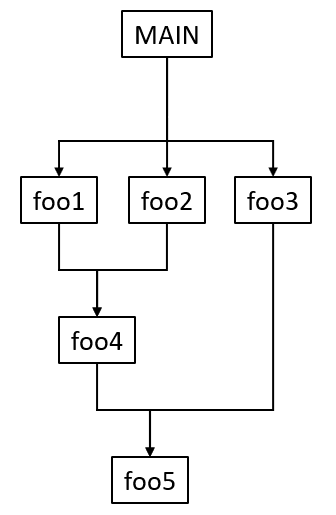
\includegraphics[scale=0.5]{images/task_dependence_graph_synctasks.png}
\caption{Task dependence graph of 3.synctasks.c}
\label{task_dependence_graph_synctasks}
\end{figure}

\textbf{2. Rewrite the program using only taskwait as task synchronisation mechanism (no depend clauses allowed)}
\subsubsection{4.taskloop.c}
\textbf{1. Find out how many tasks and how many iterations each task execute when using the grainsize
and num tasks clause in a taskloop. You will probably have to execute the program several times in order to have a clear answer to this question.}
\textbf{2. What does occur if the nogroup clause in the first taskloop is uncommented?}

\section{Observing overheads}
In this last section we will be observing the main results obtained in terms of overheads for \textit{parallel},\textit{task} and the different synchronisation mechanisms. We will discuss our conclusions and support them with tables and plots.

\subsection{Thread creation and termination}
In this part we will learn about the thread creation and termination overhead and how it varies. We will be using the \textit{pi\_omp\_parallel.c} file, which it computes the difference of time between the sequential execution and the parallel execution when using a certain number of threads and finally uses that information to print the difference in time (in microseconds), which is the overhead introduced by the parallel construct. 
\\
\medskip
In the results of the execution we can see that the order of magnitude of the overhead generated is in microseconds, we can see it clearly in figure \ref{piqueue}, when the execution starts, the first message informs about it. 
\\
Observing the results on the execution of \textit{pi\_omp\_parallel} with just 1 iteration and a maximum of 24 threads, see in figure \ref{overheadplot1}, we can confirm that the time of the overhead is not constant, it increases linearly when the number of threads increase. Moreover, the overhead per thread tends to decrease because when the number of threads increases every thread has to do less calculations.

\begin{figure}[H]
\centering
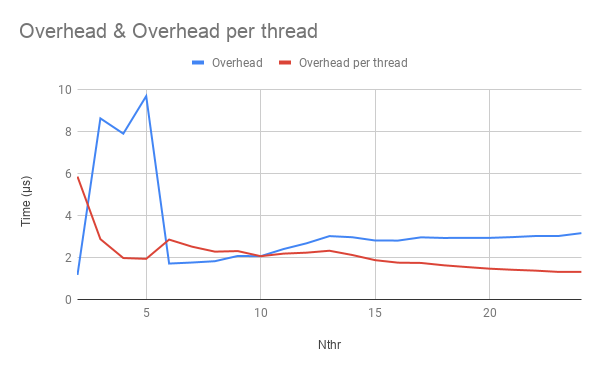
\includegraphics[scale=0.5]{images/thread.png}
\caption{Plot of the overhead and overhead per thread depending on the number of threads}
\label{overheadplot1}
\end{figure}


\begin{figure}[H]
\begin{lstlisting}[frame=single]
par4111@boada-1:~/lab2/overheads$ qsub -l execution submit-omp.sh pi_omp_parallel 1 24
Your job 97651 ("submit-omp.sh") has been submitted

par4111@boada-1:~/lab2/overheads$ more pi_omp_parallel_1_24.txt 
All overheads expressed in microseconds
Nthr	Overhead	Overhead per thread
2	1.1726		0.5863
3	0.8639		0.2880
4	0.7910		0.1978
5	0.9701		0.1940
6	1.7148		0.2858
7	1.7640		0.2520
8	1.8267		0.2283
9	2.0780		0.2309
10	2.0664		0.2066
11	2.4082		0.2189
12	2.6808		0.2234
13	3.0237		0.2326
14	2.9701		0.2122
15	2.8141		0.1876
16	2.8110		0.1757
17	2.9655		0.1744
18	2.9356		0.1631
19	2.9420		0.1548
20	2.9402		0.1470
21	2.9768		0.1418
22	3.0285		0.1377
23	3.0284		0.1317
24	3.1657		0.1319

\end{lstlisting}
\caption{Execution of pi\_omp\_parallel.c with 1 iteration and a maximum of 24 threads}
\label{piqueue}
\end{figure}
\subsection{Task creation and synchronization}
In this part we will learn about the overhead related to the creation of \textbf{tasks} and their synchronization at \textbf{taskwait} and how it varies. We will be using the \textit{pi\_omp\_tasks.c} file, which it computes the difference of time between the sequential execution and the version that creates the tasks, when using a certain number of tasks and finally uses that information to print the difference in time (in microseconds), which is the overhead introduced by the \textbf{task} and \textbf{taskwait} constructs. 
\\
\medskip
In the results of the execution we can see that the order of magnitude of the overhead generated is in microseconds, we can see it clearly in figure \ref{piqueuetask}, when the 
execution starts, the first message informs about it. 
\\
\medskip

Observing the results on the execution of \textit{pi\_omp\_tasks} with 10 iterations and 1 thread, see figure \ref{overheadplot2}, we can confirm that the time of the overhead does not depend on the number of tasks. The overhead will cost the same independently of the number of tasks, so it is constant. This affirmation is defended mainly by the tiny variation of time, probably given by the inestability of the machine. 
\\
\bigskip

\begin{figure}[H]
\centering
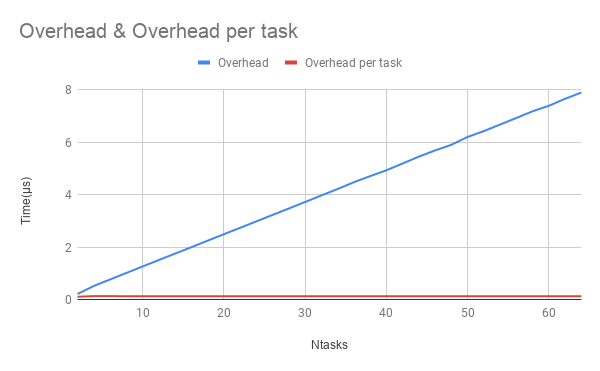
\includegraphics[scale=0.5]{images/task.png}
\caption{Plot of the overhead and overhead per task depending on the number of tasks}
\label{overheadplot2}
\end{figure}



\begin{figure}[H]
\begin{lstlisting}[frame=single]
par4111@boada-1:~/lab2/overheads$ qsub -l execution submit-omp.sh pi_omp_tasks 10 1
Your job 97659 ("submit-omp.sh") has been submitted
par4111@boada-1:~/lab2/overheads$ more pi_omp_tasks_10_1.txt 
All overheads expressed in microseconds
Ntasks	Overhead	Overhead per task
2	0.2105		0.1052
4	0.5151		0.1288
6	0.7635		0.1273
8	1.0115		0.1264
10	1.2594		0.1259
12	1.5057		0.1255
14	1.7508		0.1251
16	1.9950		0.1247
18	2.2435		0.1246
20	2.4908		0.1245
22	2.7343		0.1243
24	2.9798		0.1242
26	3.2272		0.1241
28	3.4727		0.1240
30	3.7192		0.1240
32	3.9713		0.1241
34	4.2150		0.1240
36	4.4738		0.1243
38	4.7067		0.1239
40	4.9300		0.1232
42	5.1890		0.1235
44	5.4513		0.1239
46	5.6880		0.1237
48	5.9030		0.1230
50	6.2037		0.1241
52	6.4264		0.1236
54	6.6773		0.1237
56	6.9273		0.1237
58	7.1824		0.1238
60	7.3931		0.1232
62	7.6592		0.1235
64	7.8985		0.1234
\end{lstlisting}
\caption{Execution of pi\_omp\_tasks.c with 10 iteration and 1 thread}
\label{piqueuetask}
\end{figure}


\section{Conclusions}
Jo borraria lo de conlusions, fa tot el pal escriure-ho



\end{document}